\documentclass[11pt,a4paper]{article}
\usepackage[margin=2.05cm]{geometry}
\usepackage{setspace}
\setstretch{1.0}
\usepackage{amsmath,amssymb}
\usepackage{booktabs}
\usepackage{siunitx}
\usepackage{tikz}
\usetikzlibrary{arrows.meta}
\usepackage{graphicx}
\usepackage[hidelinks]{hyperref}

\title{Singulation-Constrained Terrain Coverage\\for a Wooden Seed-Planting Machine}
\author{System Design Study\\[0.3em]
\large Short paper on the second innovation of the wooden seed-planter thesis}
\date{}

\begin{document}
\maketitle

\begin{abstract}
Coverage planners for seeding choose a heading to save energy on a slope. Metering measurements show that the same machine loses seeds when it accelerates or when the seed interval becomes shorter than the sensing delay. On a timber row unit there is a further excluded speed, near the resonance of the arm. This paper puts those limits inside coverage. An outer search picks a heading and a steady speed inside the set the meter can still repair. An inner linear time-varying predictive tracker may slow down for a headland and may not enter the resonant interval or authorise a late repair. On a \(1.44\,\mathrm{ha}\) rectangle at an eight-percent grade, the search returns \(55^\circ\) from uphill at \(1.4\,\mathrm{m/s}\). Modelled non-conservative work falls by about \(7.7\%\) relative to an open-loop uphill plan, and the failed-placement fraction falls from \(0.56\) to \(0.07\).
\end{abstract}

\noindent\textbf{Keywords:} coverage planning, model predictive control, seeding, terrain, wooden planter.

\section{Introduction}
Field coverage is usually stated as a geometric problem: paint a polygon with straight swaths, turn on a headland, and keep the non-working distance small \cite{choset2001,oksanen2009,bochtis2008}. On a slope the heading is no longer only a statement about how many turns fit along the short side. Grade changes the non-conservative work of rolling and slip, and three-dimensional coverage has reduced seeding energy by up to about \(10\) to \(16\%\) on sample fields by choosing the driving direction \cite{jin2011,vahdanjoo2023}. Trackers that follow the resulting path are now routinely predictive. They can respect steering rate, estimate the state they control, and even carry an efficiency term inside the horizon rather than tracking a frozen path so faithfully that the job takes longer \cite{backman2012,kraus2013,plessen2017,xu2022}.

A planter adds a constraint those planners do not carry. Seed singulation of an electric-drive meter stayed near \(98\%\) in steady running and worsened when speed changed quickly or when the meter was asked for too many seeds per minute \cite{mangus2017}. A vision repair that is accurate and late increases misses \cite{borja2021}. The companion metering design for this machine publishes a feasible speed set from that delay and from the resonance of a laminated row unit. This paper is the coverage half. It minimises work, time and failed placements, and it treats the feasible set as a hard constraint. Efficiency may choose among admissible speeds. It may not define admissibility.

The split follows the usual time scales. Heading is chosen before motion, or when the machine is stopped. Steering and speed are chosen every tenth of a second. Plate speed stays on the row and uses the realised ground speed, not the speed the plan hoped for a second earlier. Using the request instead of the realisation bunches seeds at the start of a swath whenever the wheels are still slow.

\section{Cost on a grade}
Only non-conservative work enters the ledger. A vehicle that drives up a slope and later drives down it returns gravitational potential. It does not return rolling resistance, slip loss or drag. With mass \(M\), rolling coefficient \(C_{rr}\), slip coefficient \(C_s\), drivetrain efficiency \(\eta_d\) and heading \(\beta\) measured from uphill,
\begin{equation}
\label{eq:work}
\begin{aligned}
\Gamma(\beta)&=1+\gamma\cos^2\beta,\\
F&=C_{rr}Mg\cos\alpha+C_s Mg\sin^2\alpha\,\Gamma(\beta)\\
&\quad+\tfrac12\rho C_dA\,v^2.
\end{aligned}
\end{equation}
Work along a swath is \(F v/\eta_d\) integrated in distance. The coefficients used here are \(M=460\,\mathrm{kg}\), \(C_{rr}=0.085\), \(C_s=2\), \(\gamma=1.15\) and \(\eta_d=0.70\). They are chosen so that an eight-percent grade changes work by several percent, the same order as published direction savings, without copying a percentage from another field \cite{vahdanjoo2023}. Drag at these speeds is about a newton and does not decide the heading.

Turns are not free. Each swath ends in a turn of radius \(4.2\,\mathrm{m}\), driven at \(0.8\,\mathrm{m/s}\), with an extra eight percent on the force. A heading with short rows buys a lower grade factor and pays more turns. The distance spent accelerating at each end of a row, at \(0.7\,\mathrm{m/s}^2\), is charged with the meter's accelerated miss model rather than with the steady model. Short rows therefore hurt singulation only when that fraction becomes large. At \(1.5\,\mathrm{m/s}\) on a \(180\,\mathrm{m}\) row the fraction is under two percent. On an \(80\,\mathrm{m}\) row it is about four percent. Heading is an energy and time decision inside the singulation plateau, and a singulation decision only near the plateau's edge.

The failure term mixes misses, half the multiples, and a depth survival \(\exp(-\sigma_z^2/(2\cdot 6.5^2))\) with \(\sigma_z\) in millimetres. The half-weight treats a multiple as wasted seed that is not always a total loss. The survival curve encodes a narrow depth band. Both are estimation choices, not a measured germination function. They are the same function for every plan, so a ranking is not an artefact of a special penalty on one baseline.

Candidates are discarded before the scalar cost is compared if the modelled quality-of-feed index is below \(0.955\) or the depth root-mean-square error is above \(4\,\mathrm{mm}\), and if the speed lies in the resonant interval from \(2.15\) to \(2.55\,\mathrm{m/s}\). The scalar cost then adds work, a time weight of \(0.55\,\mathrm{MJ}\) per hour, and a failure weight that makes a failed placement expensive beside the few tenths of a megajoule that separate headings. Changing the weights moves the choice among feasible plans. It does not move the filter.

\begin{figure}[t]
\centering
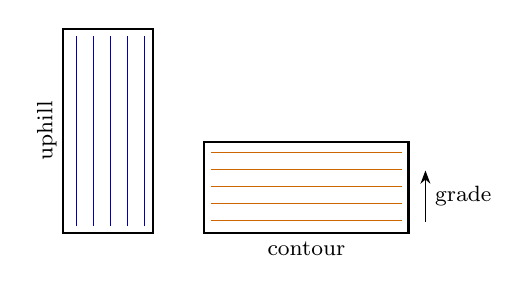
\begin{tikzpicture}[scale=0.72, font=\footnotesize, >=Stealth]
  \draw[thick] (0,0) rectangle (1.6,3.6);
  \foreach \x in {0.25,0.55,0.85,1.15,1.45}
    \draw[blue!70!black] (\x,0.12) -- (\x,3.48);
  \node[rotate=90] at (-0.28,1.8) {uphill};
  \begin{scope}[xshift=2.5cm]
    \draw[thick] (0,0) rectangle (3.6,1.6);
    \foreach \y in {0.22,0.52,0.82,1.12,1.42}
      \draw[orange!80!black] (0.12,\y) -- (3.48,\y);
    \node at (1.8,-0.28) {contour};
  \end{scope}
  \draw[->] (6.4,0.2) -- (6.4,1.1) node[midway,right] {grade};
\end{tikzpicture}
\caption{The same rectangle. Long uphill rows pay slip. Short contour rows pay a turn, and an acceleration, on every swath.}
\label{fig:field}
\end{figure}

\section{Search and tracker}
Headings are searched from uphill to contour. Speeds are searched in steps of \(0.1\,\mathrm{m/s}\) inside the meter's feasible set. For each pair the work, time, accelerated fraction and failure probability are closed forms. The swath joins are then smoothed so curvature and curvature rate stay inside the steering limits \cite{plessen2017}. If no speed profile on the join keeps the repair fraction at or above \(0.85\), the headland is lengthened. Unplanted edge is counted as missed seed, so a planner cannot hide a singulation problem by calling it headland.

The tracker linearises the kinematic bicycle, plus longitudinal acceleration, about the reference every \(100\,\mathrm{ms}\) \cite{rajamani2012,plessen2017}. The horizon is \(1.5\,\mathrm{s}\), fifteen steps. Lateral error is weighted more than longitudinal error, because a drifted row plants the neighbour's strip, whereas a lag along the row is removed by the plate once the realised speed is known. Speed error in the tracking cost is light. Speed is already constrained. The hard constraints are the feasible set, acceleration and steering limits, the steering rate, and the repair-fraction inequality. A quadratic bowl penalises speed inside the resonant interval even though that interval is already excluded, so a disturbance cannot cross it for free. The program is a convex quadratic program solved by an active-set method suitable for the sample period \cite{ferreau2014,mayne2000}.

A feasible reference in the interior of the constraints, with slip smaller than the margin between the working speed and the edge of the feasible set, keeps the shifted previous solution feasible. At \(1.4\,\mathrm{m/s}\) against a latency edge near \(1.87\,\mathrm{m/s}\), that margin is about \(0.47\,\mathrm{m/s}\). If a steeper patch consumes it, the tracker brakes. Braking stays feasible because a lower speed improves the repair test and moves away from resonance. The on-line seed spacing is logged for the seed map \cite{griepentrog2005}. It is not a hard constraint. It arrives about one flight time late, which is the wrong signal to require at the current step.

A prescription that shortens the spacing also shortens the hole period and therefore shrinks the feasible set. The search lowers speed on the dense patch before the tracker runs. It does not rotate the field heading for a constraint a speed change already meets. The plate never receives a speed command that bypasses the repair test.

\section{Estimation on one rectangle}
The field is \(80\,\mathrm{m}\) across the slope and \(180\,\mathrm{m}\) along it, so a contour heading has short rows and an uphill heading has long ones. The grade is eight percent. The area is \(1.44\,\mathrm{ha}\). Three plans use the same work model and the same flexure. The first is an open-loop plate at \(1.6\,\mathrm{m/s}\) straight uphill. The second is the same heading at \(2.4\,\mathrm{m/s}\), on the timber resonance. The third is the search result.

\begin{table}[t]
\centering
\caption{Plans on the estimation field. The third row is the constrained search.}
\label{tab:plans}
\begin{tabular}{@{}lrrrr@{}}
\toprule
Plan & Work & Time & QFI & Fail \\
 & (MJ) & (h) & & \\
\midrule
Open, uphill, \(1.6\,\mathrm{m/s}\) & 4.78 & 1.22 & 0.808 & 0.561 \\
Open, uphill, \(2.4\,\mathrm{m/s}\) & 4.80 & 0.86 & 0.652 & 0.998 \\
\(55^\circ\), \(1.4\,\mathrm{m/s}\) & 4.42 & 1.41 & 0.978 & 0.068 \\
\bottomrule
\end{tabular}
\end{table}

Table~\ref{tab:plans} is the comparison. Work falls from \(4.78\,\mathrm{MJ}\) to \(4.42\,\mathrm{MJ}\), about \(7.7\%\). Time rises from \(1.22\,\mathrm{h}\) to \(1.41\,\mathrm{h}\). The failed-placement fraction falls from \(0.56\) to \(0.07\). The resonant plan is the fastest and, under the depth curve, agronomically empty: the open-loop depth error at \(2.4\,\mathrm{m/s}\) is about \(22\,\mathrm{mm}\). Most of the index gain is available from the metering loop alone, on a fixed uphill heading, at a feasible speed. The coverage layer moves that same metering performance onto a heading that costs less work. It keeps the gain only because it is forbidden to spend the saving on a higher speed.

At \(1.5\,\mathrm{m/s}\) the uphill heading costs \(4.78\,\mathrm{MJ}\) and the \(55^\circ\) heading \(4.42\,\mathrm{MJ}\). The pure contour costs \(4.45\,\mathrm{MJ}\) and takes longer, because \(75\) turns replace \(34\). The search therefore stops short of the contour. The turn term, not a preference for oblique driving as such, breaks the tie. Turn the rectangle so the long side lies on the contour and both work and time prefer the contour: about \(4.16\,\mathrm{MJ}\) and \(1.37\,\mathrm{h}\) against about \(5.12\,\mathrm{MJ}\) and \(1.53\,\mathrm{h}\) uphill, at the same \(1.4\,\mathrm{m/s}\). The speed ceiling does not move. The heading result is a property of which side is long.

The \(7.7\%\) gap is a little below the \(9.5\) to \(15.6\%\) direction savings reported on other seeding fields \cite{vahdanjoo2023}. This rectangle is a moderate grade with a slip term that does not dominate rolling resistance. In energy units the prize is about \(0.10\,\mathrm{kWh}\) on \(1.44\,\mathrm{ha}\). The singulation and depth columns are where the plan changes the operation by a factor rather than by a fraction. A contract that pays for time alone prefers the open-loop uphill run. A contract that pays for established plants prefers the constrained plan even before the energy line is read \cite{pedersen2006}.

\section{A headland, and the tracker cost}
The stage cost is tracking error plus a light input penalty, a weight on the failure probability at the predicted speed and acceleration, and the resonant bowl. Lateral error dominates the tracking term. On a straight swath at \(1.4\,\mathrm{m/s}\) with a \(1.6\,\mathrm{m}\) wheelbase, a steering step of \(0.05\,\mathrm{rad}\) changes heading by about \(0.004\,\mathrm{rad}\) in one \(100\,\mathrm{ms}\) sample and lateral position by well under a centimetre on the next sample. The horizon is long enough to see a growing lateral error and short enough that the linearisation is recomputed before the vehicle has wrapped a turn inside one linear model. The turn itself lives in the smoothed reference. Freezing the linearisation for a whole headland would be a linear controller about the wrong point.

Consider the brake from \(1.4\,\mathrm{m/s}\) to the turn speed \(0.8\,\mathrm{m/s}\) at \(0.7\,\mathrm{m/s}^2\). The distance required is \((1.4^2-0.8^2)/(2\cdot 0.7)=0.94\,\mathrm{m}\), about eight to ten tracker steps, inside the \(1.5\,\mathrm{s}\) horizon. The repair fraction at that speed and acceleration remains \(1\), because the hole period is \(0.143\,\mathrm{s}\) and the acceleration surcharge is only about \(8\,\mathrm{ms}\). A pure time-optimal tracker would postpone the brake and then brake harder. A \(1.2\,\mathrm{m/s}^2\) brake saves a fraction of a second and drops the repair fraction toward \(0.7\). The hard constraint forbids that brake. During an unplanted headland the plate is inhibited rather than asked to singulate with the boot out of the soil. On the next swath the depth integral is released, and the plate follows realised speed so the first metre is not bunched.

If a solve exceeds the \(40\,\mathrm{ms}\) budget inside the \(100\,\mathrm{ms}\) sample, the tracker applies the next move of the previous feasible solution. A hold remains feasible. An infeasible scramble does not. The warm start is the shifted previous solution with the terminal linear-quadratic move appended.

\section{What moves the plan, and what does not}
Per hectare the constrained plan uses about \(3.1\,\mathrm{MJ}\) and about \(0.98\,\mathrm{h}\), with a failed-placement fraction of \(0.07\). The open-loop uphill plan at \(1.6\,\mathrm{m/s}\) uses about \(3.3\,\mathrm{MJ}\) and about \(0.85\,\mathrm{h}\), with a failed-placement fraction of \(0.56\). The energy prize on the whole field is about \(0.10\,\mathrm{kWh}\). It is a direction effect of a few percent on a moderate grade, consistent in kind with published direction savings and smaller than those reported on steeper sample fields. The factor-of-eight drop in the failure fraction is the reason to accept the extra quarter of an hour. That factor inherits the depth curve. A species that tolerates \(7\,\mathrm{mm}\) of depth error would shrink the gap. A species as shallow as the spinifex optimum near \(5\,\mathrm{mm}\) would enlarge it and would also tighten the \(4\,\mathrm{mm}\) ceiling.

Three specification changes move different columns, which is how the two technologies stay separable. Doubling the timber stiffness raises the natural frequency by \(\sqrt{2}\) and pushes resonance out past the speeds a planter is likely to ask for. The latency cut remains. A late detector, with inference at \(40\,\mathrm{ms}\) instead of \(14\,\mathrm{ms}\), shrinks the plateau from the right and the search returns a slower speed, or no plan if the plateau disappears. Doubling the grade widens the work gap between uphill and oblique headings and does not move the metering table. A field trial that found a larger energy difference and the same speed ceiling would be confirming that split. A trial that found no resonant peak would recompute the forbidden interval from the measured frequency. It would not delete the interval after one smooth run.

The rotated rectangle, long side on the contour, is the check that \(55^\circ\) is not a universal answer. There the contour wins both work and time, and the search agrees with a pure energy planner. The speed remains \(1.4\,\mathrm{m/s}\) because nothing in the rotation changes the delay or the natural frequency. Heading is a property of which side is long. The speed ceiling travels.

\section{Conclusion}
Singulation-constrained coverage chooses heading and speed inside the set a vision meter can still repair, and it keeps the timber resonance out of steady running. On the estimation rectangle the selected plan is \(55^\circ\) from uphill at \(1.4\,\mathrm{m/s}\), with a small work reduction against an uphill baseline and a large reduction in modelled failed placements. A faster resonant plan wins the clock and fails the depth band. The figures are evaluations of a declared model. Replacing the rolling coefficient, the delay, or the depth curve changes the numbers. It does not give the tracker a private speed set.

\begin{thebibliography}{14}
\bibitem{choset2001}
H.~Choset, ``Coverage for robotics---A survey of recent results,'' \emph{Ann. Math. Artif. Intell.}, vol.~31, pp.~113--126, 2001.
\bibitem{oksanen2009}
T.~Oksanen and A.~Visala, ``Coverage path planning algorithms for agricultural field machines,'' \emph{J. Field Robot.}, vol.~26, no.~8, pp.~651--668, 2009.
\bibitem{bochtis2008}
D.~D. Bochtis and S.~G. Vougioukas, ``Minimising the non-working distance travelled by machines operating in a headland field pattern,'' \emph{Biosyst. Eng.}, vol.~101, no.~1, pp.~1--12, 2008.
\bibitem{jin2011}
J.~Jin and L.~Tang, ``Coverage path planning on three-dimensional terrain for arable farming,'' \emph{J. Field Robot.}, vol.~28, no.~3, pp.~424--440, 2011.
\bibitem{vahdanjoo2023}
M.~Vahdanjoo, R.~Gislum, and C.~A.~G. S{\o}rensen, ``Three-dimensional area coverage planning for a seeding operation,'' SSRN 4594418, 2023.
\bibitem{backman2012}
J.~Backman, T.~Oksanen, and A.~Visala, ``Navigation system for agricultural machines: Nonlinear model predictive path tracking,'' \emph{Comput. Electron. Agric.}, vol.~82, pp.~32--43, 2012.
\bibitem{kraus2013}
T.~Kraus \emph{et al.}, ``Moving horizon estimation and nonlinear model predictive control for autonomous agricultural vehicles,'' \emph{Comput. Electron. Agric.}, vol.~98, pp.~25--33, 2013.
\bibitem{plessen2017}
M.~M. Graf~Plessen and A.~Bemporad, ``Reference trajectory planning under constraints and path tracking using linear time-varying model predictive control for agricultural machines,'' \emph{Biosyst. Eng.}, vol.~153, pp.~28--41, 2017.
\bibitem{xu2022}
J.~Xu, J.~Lai, R.~Guo, and X.~Lu, ``Efficiency-oriented MPC algorithm for path tracking in autonomous agricultural machinery,'' \emph{Agronomy}, vol.~12, no.~7, 1662, 2022.
\bibitem{mangus2017}
D.~L. Mangus \emph{et al.}, ``Development of high-speed camera hardware and software to evaluate real-time electric seed meter accuracy,'' \emph{Comput. Electron. Agric.}, vol.~142, pp.~314--325, 2017.
\bibitem{borja2021}
A.~A. Borja, R.~M. Amongo, D.~C. Suministrado, and J.~P. Pabico, ``Design and evaluation of a machine vision system and mechatronic drive for a pneumatic seed meter for corn,'' \emph{Philipp. J. Agric. Biosyst. Eng.}, 2021.
\bibitem{rajamani2012}
R.~Rajamani, \emph{Vehicle Dynamics and Control}, 2nd~ed. Springer, 2012.
\bibitem{ferreau2014}
H.~J. Ferreau, C.~Kirches, A.~Potschka, H.~G. Bock, and M.~Diehl, ``qpOASES: A parametric active-set algorithm for quadratic programming,'' \emph{Math. Program. Comput.}, vol.~6, no.~4, pp.~327--363, 2014.
\bibitem{mayne2000}
D.~Q. Mayne, J.~B. Rawlings, C.~V. Rao, and P.~O.~M. Scokaert, ``Constrained model predictive control: Stability and optimality,'' \emph{Automatica}, vol.~36, no.~6, pp.~789--814, 2000.
\bibitem{griepentrog2005}
H.~W. Griepentrog, M.~N{\o}rremark, H.~Nielsen, and B.~S. Blackmore, ``Seed mapping of sugar beet,'' \emph{Precis. Agric.}, vol.~6, pp.~157--165, 2005.
\bibitem{pedersen2006}
S.~M. Pedersen, S.~Fountas, H.~Have, and B.~S. Blackmore, ``Agricultural robots---System analysis and economic feasibility,'' \emph{Precis. Agric.}, vol.~7, pp.~295--308, 2006.
\end{thebibliography}

\end{document}
